\documentclass[a4paper]{article}

\usepackage[margin=0mm]{geometry}
\usepackage[T1]{fontenc}
\usepackage{lmodern}
\usepackage[dvipsnames]{xcolor}
\usepackage{siunitx}
\usepackage{tikz}

\pagestyle{empty}
\setlength{\parindent}{0pt}

\definecolor{ray00}{HTML}{A33A32}
\definecolor{ray01}{HTML}{C46A20}
\definecolor{ray02}{HTML}{A48716}
\definecolor{ray03}{HTML}{4F8129}
\definecolor{ray04}{HTML}{18706A}
\definecolor{ray05}{HTML}{286B9E}
\definecolor{ray06}{HTML}{4D58A5}
\definecolor{ray07}{HTML}{76509A}
\definecolor{ray08}{HTML}{9A4677}

\begin{document}

\centering
\vspace*{\fill}
  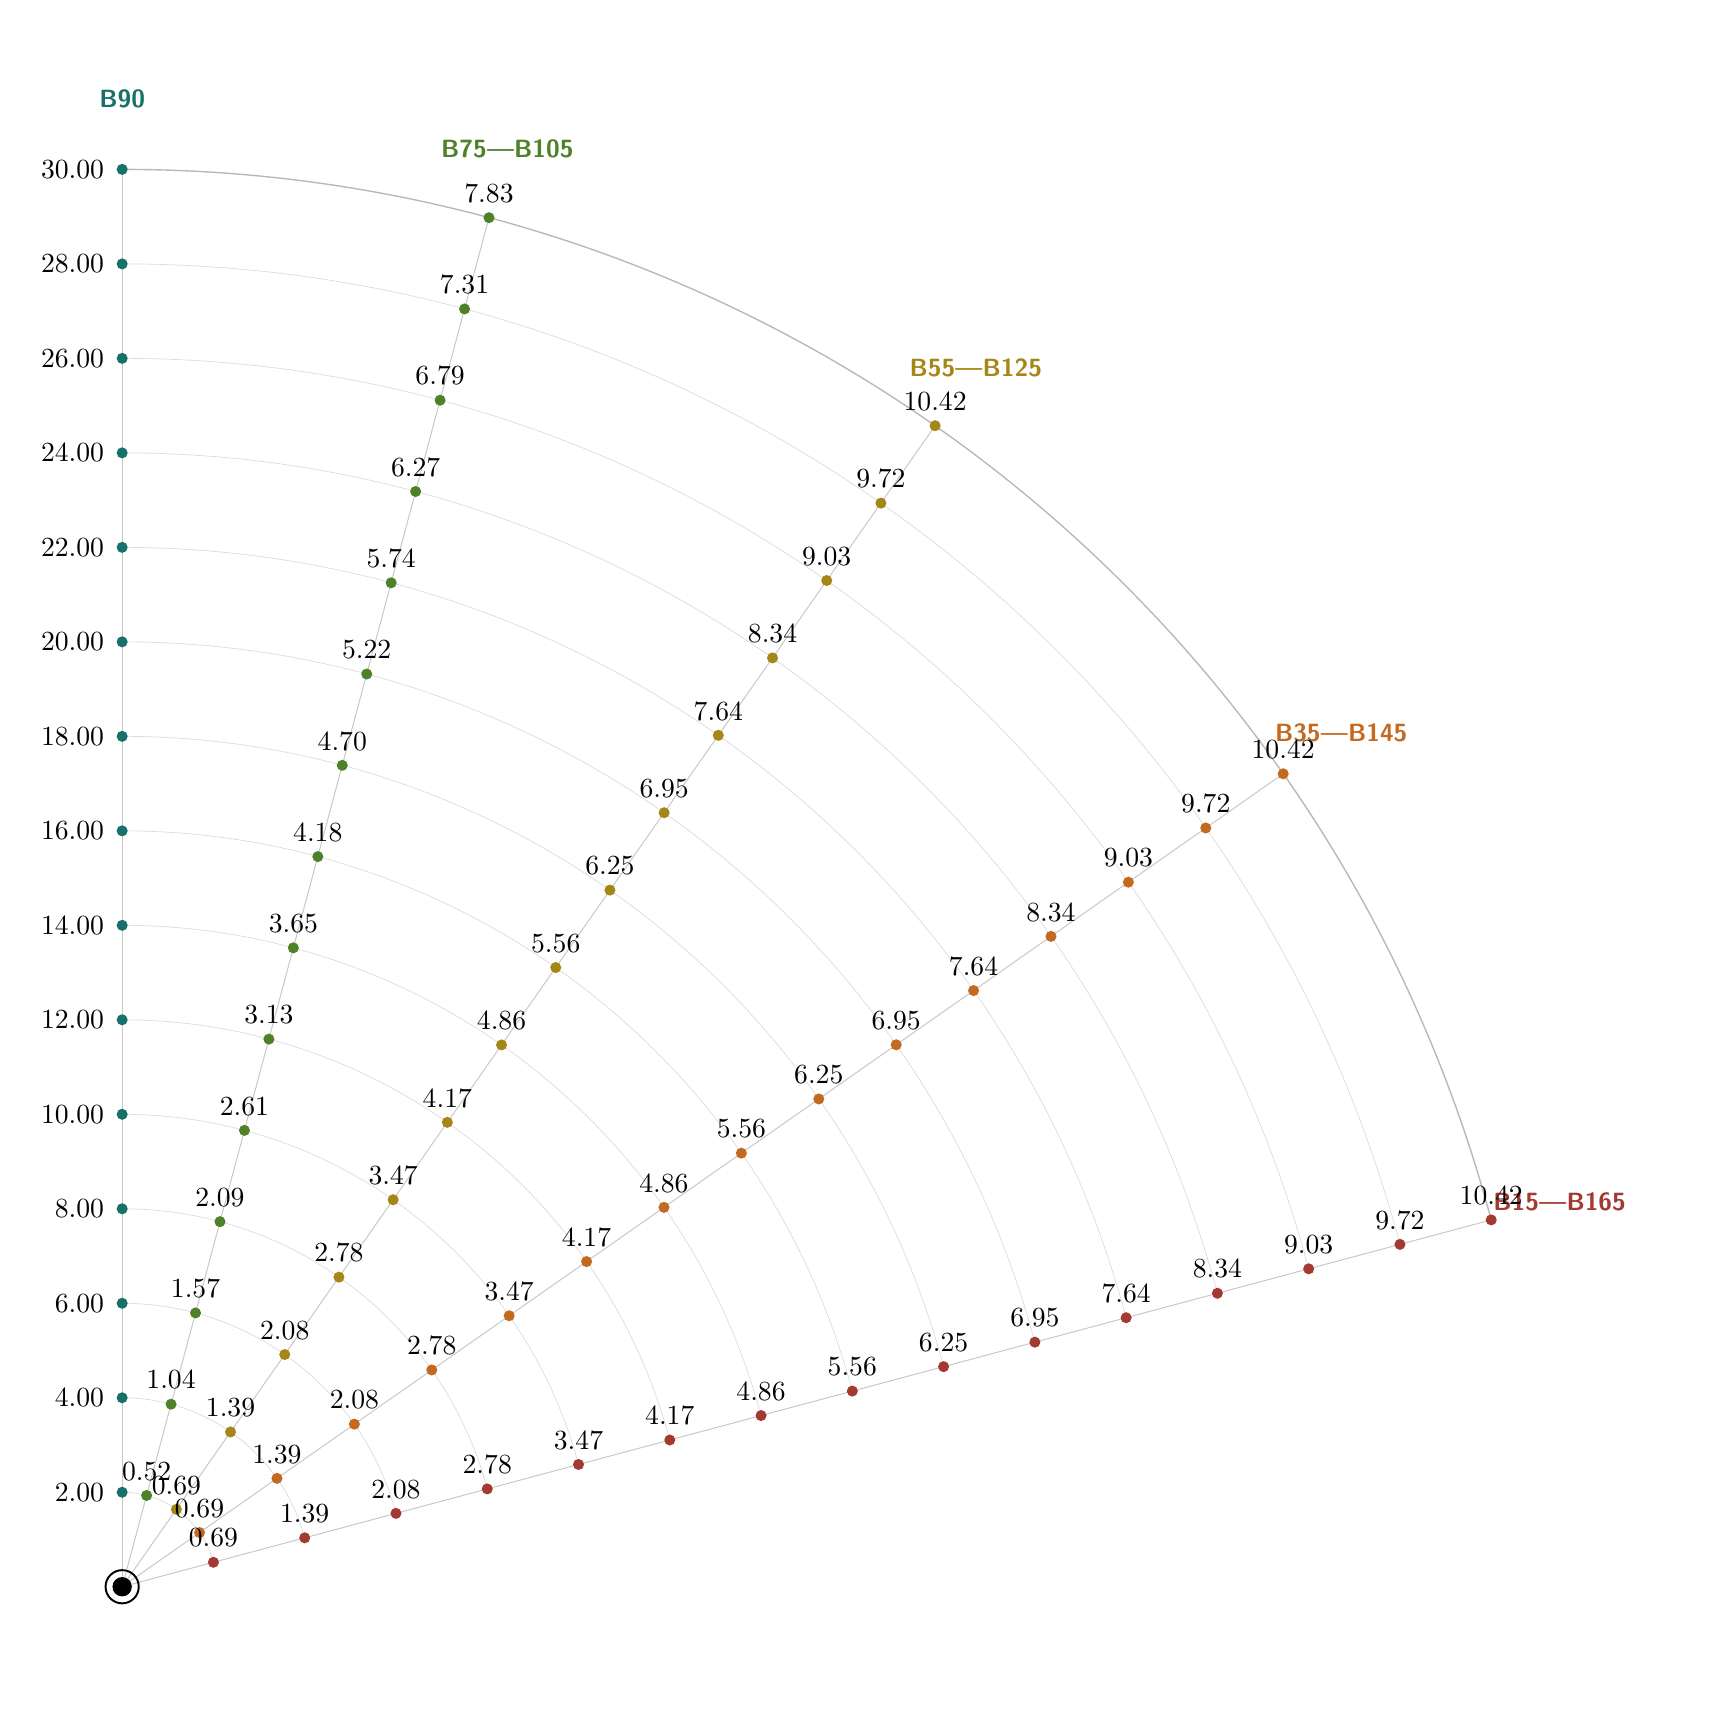
\begin{tikzpicture}[x=0.6cm,y=0.6cm]
    \path[use as bounding box] (-2,-2) rectangle (33,33);

    % Concentric sampling arcs group points at the same radial distance.
    \foreach \radius in {2,4,...,28} {
      \draw[black!14, line width=0.25pt]
        (15:\radius) arc[start angle=15,end angle=90,radius=\radius];
    }
    \draw[black!28, line width=0.5pt]
      (15:30) arc[start angle=15,end angle=90,radius=30];

    % Subtle radial guides connect each bearing to the node.
    \foreach \bearing in {15,35,55,75,90} {
      \draw[black!22, line width=0.35pt] (0,0) -- (\bearing:30);
    }

    % Nine bearings, each sampled at 2, 4, ..., 30 metres.
    \foreach \bearing/\pointcolor in {15/ray00,35/ray01,55/ray02,
      75/ray03,90/ray04} {
      \foreach \radius in {2,4,...,30} {
        \fill[\pointcolor] (\bearing:\radius) circle[radius=2pt];
      }
    }

    \foreach \bearing/\pointcolor/\bearingname in {15/ray00/B15|B165,
      35/ray01/B35|B145,55/ray02/B55|B125,75/ray03/B75|B105,
      90/ray04/B90} {
      \node[\pointcolor, font=\sffamily\bfseries\small]
        at (\bearing:31.5) {\bearingname};
    }

    \foreach \radius in {2,4,...,30} {
      \node[black, font=\sffamily\normalsize, anchor=east, xshift=-3pt]
        at (90:\radius) {\num[mode=text,minimum-decimal-digits=2]{\radius}};
    }

    \foreach \radius in {2,4,...,30} {
      \node[black, font=\sffamily\normalsize, anchor=south, yshift=2pt]
        at (75:\radius) {\num[mode=text,round-mode=places,
          round-precision=2,minimum-decimal-digits=2]
          {\fpeval{2*\radius*sin(7.5*pi/180)}}};
    }

    \foreach \radius in {2,4,...,30} {
      \node[black, font=\sffamily\normalsize, anchor=south, yshift=2pt]
        at (55:\radius) {\num[mode=text,round-mode=places,
          round-precision=2,minimum-decimal-digits=2]
          {\fpeval{2*\radius*sin(10*pi/180)}}};
    }

    \foreach \bearing in {35,15} {
      \foreach \radius in {2,4,...,30} {
        \node[black, font=\sffamily\normalsize, anchor=south, yshift=2pt]
          at (\bearing:\radius) {\num[mode=text,round-mode=places,
            round-precision=2,minimum-decimal-digits=2]
            {\fpeval{2*\radius*sin(10*pi/180)}}};
      }
    }

    % Logical origin of the experiment.
    \fill[black] (0,0) circle[radius=3.5pt];
    \draw[black, line width=0.7pt] (0,0) circle[radius=6pt];
  \end{tikzpicture}
\par\vspace{4mm}
\begin{minipage}{0.88\paperwidth}
  \sffamily\small
  \textbf{PREPARAZIONE DEL CAMPO}\par\vspace{2mm}
  \begin{enumerate}
    \setlength{\itemsep}{1.5mm}
    \setlength{\parskip}{0pt}
    \setlength{\topsep}{0pt}
    \item Fissare il node nell'origine \textbf{O}, mantenendone invariati posizione e orientamento.
    \item Tracciare \textbf{B90}. Partendo da O, segnare le distanze da \SI{2}{m} a
      \SI{30}{m}, con incrementi di \SI{2}{m}.
    \item A ogni distanza, individuare \textbf{B75} usando la quota riportata rispetto a B90.
      Proseguire in sequenza: \textbf{B55} da B75, \textbf{B35} da B55 e
      \textbf{B15} da B35.
    \item Riflettere gli stessi punti rispetto a B90 per ottenere \textbf{B105},
      \textbf{B125}, \textbf{B145} e \textbf{B165}. Ogni punto riflesso deve mantenere
      la stessa distanza da O.
    \item Prima dell'acquisizione, verificare distanza e bearing selezionati, collocare ogni
      tag sul punto assegnato e mantenere per tutti i tag altezza e orientamento prescritti.
  \end{enumerate}
  \vspace{1mm}
  \noindent\colorbox{black!7}{%
    \parbox{\dimexpr\linewidth-2\fboxsep\relax}{%
      \textbf{HOTSPOT}\hfill SSID: \texttt{field-net}\hspace{8mm}
      Password: \texttt{field-net}}}
\end{minipage}
\vspace*{\fill}

\end{document}
